\chapter{Optimization for Neural Networks and CNNs}
The optimization of a NN comes with more learning. \\
The main idea is to adjust all the weights of the network $\theta$ such that the cost function is minimized. Formally:\\
\[
min_\theta \sum_i L(y_i, f(x_i, \theta))
\]

To do this, usually we use gradient descent and back propagation, although there are different methods. 
\section{Batch (Stochastic) Gradient Descent (BGD) and (SGD) }
The main idea is that the learning rate $\eta$ changes linearly. \\
The update to the weights (w) is: \\
$w = w - \eta_k g$

Pros: estimates are stable \\
Cons: needs to estimate the GD throughout the whole training.

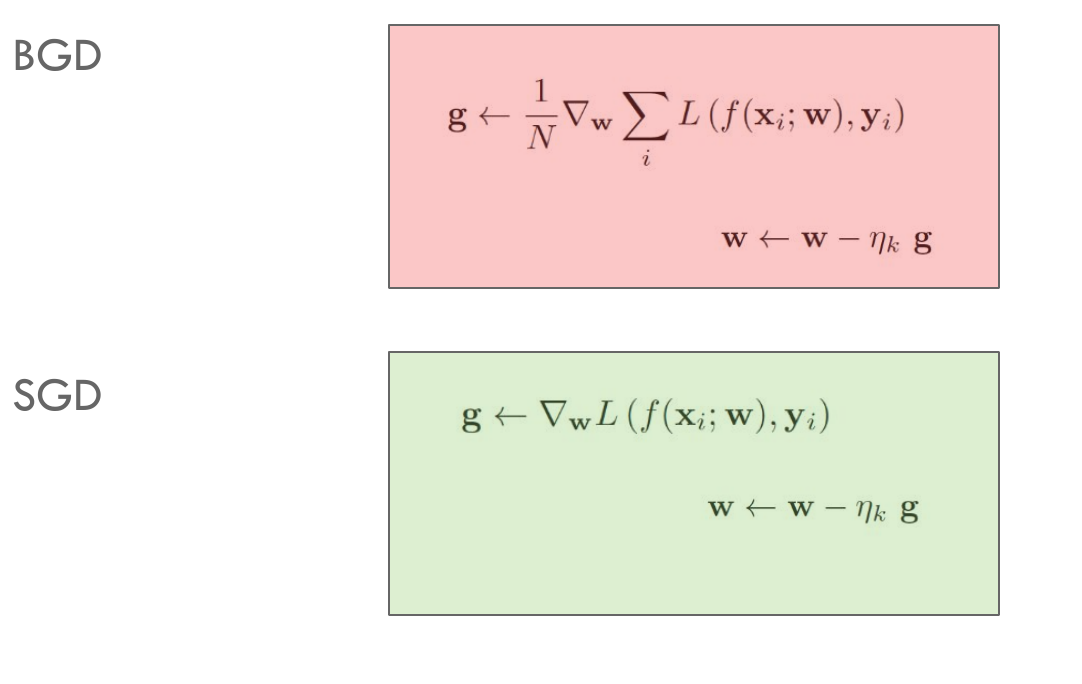
\includegraphics[scale=0.18]{bdg}

Gradient descent estimates can be very noisy so a solution is to reduce the number of batches (minibatches).\\
Another problem has to do with momentum: SGD can be very slow, so we introduce a new variable: velocity ($v$)

\section{Convolutional Neural Networks (CNNs)}
Neural networks are particularly effective when the data is spatial (i.e. language and images).

For images for instance each layer extract features from the previous output. 
\begin{definition}[Convolutional Neural Networks]
	A CNN is a neural network in which it uses convolution in at least one of its layers
\end{definition}
Okay, cool, but what is convolution? \\
Convolution is a general purpose filter operation for images. A kernel matrix is applied to images and it works by determining the central value of a pixel and adding the weights of all its neighbors.\\
In CNN's architecture there are 3 main operations:
\begin{itemize}
	\item Convolution
	\item Non-linearity
	\item Pooling
\end{itemize}

Convolution consist of learned filters. The idea is that each filter is supposed to give insight on a specific type of feature. \\
Pooling consists of reducing the spatial size of the representation: this reduces the number of parameters and controls overfitting.\\
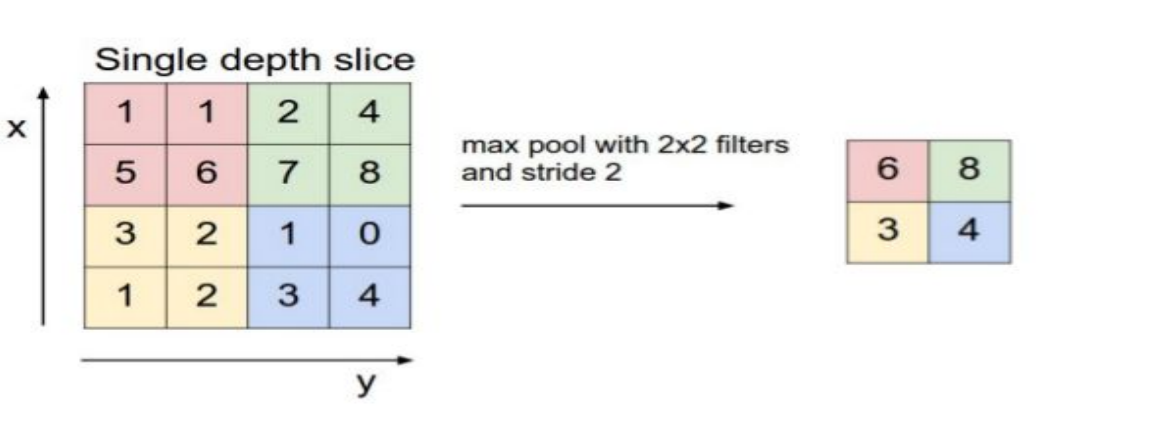
\includegraphics[scale=0.4]{pooling}
